\documentclass[12pt,a4paper]{article}
\usepackage[utf8]{inputenc}
\usepackage[russian]{babel}
\usepackage{amsmath}
\usepackage{amsfonts}
\usepackage{amssymb}
\usepackage{caption}
\usepackage{subcaption}
\usepackage{graphicx}
\usepackage{textcomp}
\author{Хасан Хафизов}
\title{Децентрализованное управление строем}

\begin{document}
	\maketitle
	\tableofcontents
\section{Введение}
C задачей совместного управления движением группы роботов чаще всего можно встретиться в военной сфере. Одним из перспективных направлений в этой области можно назвать управление группой БПЛА с целью разведки. Для этой задачи важен именно многоагентрный подход, так как для систем противовоздушной обороны (ПВО) противника поражение большого количества целей является гораздо более сложной задачей, из-за возрастания необходимых вычислительных мощностей для одновременного сопровождения множество воздушных объектов. Вероятность выполнения задачи так же повышается, так как выход из строя части роботов не окажет критического влияния на группу в целом. Дополнительный выигрыш от строевого движения можно получить задав конфигурацию строя так, чтобы за впереди идущими агентами образовывалась зона пониженного давелния, давая тем самым  возможность остальным участникам группы экономить топливо или заряд батарей.
\section{Постановка задачи}
\subsection{Описание}
В этой работе будет решаться задача управления группой роботов, объединённых в строй с произвольным порядком (рисунком). Каждый робот в строю является интеллектуальным агентом, движущимся в соответствии со своим законом управления, который направлен, во-первых на то, чтобы выполнить общую задачу, а во-вторых чтобы сохранить исходную структуру строя. В качестве задачи, которая будет выполняться строем была выбрана задача движения по произвольной траектории с задаваемой скоростою. \par
Для взаимозаменяемости требования с аппаратной точки зрения ко всем агентам однинаковые, однако программно в каждый момент времени агент будет принадлежать одному из двух классов:
\begin{itemize}
	\item Мастер — агент, задача которого отрабатывать движение по траектории и быть главным ориентиром для всех остальных агентов.
	\item Миньон — агент, задача которого сохранять своё местоположение относительно других участников группы, тем самым сохраняя структуру строя
\end{itemize}
\par
Моделирование в работе будет проводиться в горизонтальной 2D плоскости. Моделями агентов будут материальные точки с массой.
\par
Ограничения:
\begin{itemize}
	\item У каждого агента есть ограничение видимости. Если два участника строя в данный момент времени находятся вне зоны видимости друг-друга, то они не могут напрямую обмениваться информацией
	\item Максимальное по модулью управляющее воздействие ограничено
	\item Агенты передают друг-другу информацию только о своих абсолютных координатах
\end{itemize}
Основные требования к решению:
\begin{itemize}
	\item Без возмущений строй должен отрабатывать заданную траекторию с малыми погрешностями
	\item При малых возмущениях каждый отдельно взятый агент не должен существенно отколняться от своей позиции в строю. Строй в целом должен по прежнему выполнять задачу, с погрешностями соразмерными возмущениям
	\item При краткосрочных больших возмущениях, даже если строй потерял целостность, он должен самовосстанавливаться и продолжать выполнение задачи
	\item При выходе из строя одного или нескольких агентов строй должен переформироваться так, чтобы сохранить исходный рисунок
\end{itemize}
\subsection{Формальная постановка}
Вектор состояния каждого агента в горизонтальной плоскости $xy$:
$$ X = 
\begin{bmatrix}
	x_1 \\
	x_2 \\
	x_3 \\
	x_4
\end{bmatrix} ,
$$
где $x_1 = x$, $x_2 = \dot{x}$, $x_3 = y$, $x_4 = \dot{y}$. Тогда закон движения:
$$\dot{X} = AX + BU$$

\section{Алгоритм управления}
В предлагаемом мной алгоритме управления агентов можно разделить на два класса:
\begin{itemize}
	\item мастер — агент, который отрабатывает движение по траектории
	\item миньон — поддерживает своё местоположение в строю
\end{itemize}
Закон управления для этих двух типов агентов задаётся по-разному.
\subsection{Мастер}
Мастером является агент, для которого желаемый закон движения $S_d$ задаётся оператором извне: это может быть записанная в память агента траектория, целевая позиция или скорость. \par
Фактически, этот агент ничего не знает о существовании других агентов в строю (миньонов). Его задача — выполнение поставленного закона движения, поэтому закон управления зависит только от закона движения:
$$ \vec{u} = \vec{u}(S_d)$$
Рассмотрим конкретный закон управления $\vec{u}_{tr}$: движение по некоторой траектории $\vec{tr}(t)$:
$$ \vec{u}_{tr} = \vec{u}_{along} + \vec{u}_{across} $$
Закон управления состоит из двух частей. Первая $\vec{u}_{along}$ отвечает за усилие вдоль траектории, вторая $\vec{u}_{across}$ — поперёк. Направлением для $\vec{u}_{along}$ служит направление вектора между текущим положением агента и следующей точкой траектории.
\begin{center}{\textit{ (Тут будет более подробно о том, как вычисляется следующая точка траектории, о алгоритмах управления на PD регуляторах, которые используются как в $\vec{u}_{along}$, так и в $\vec{u}_{across}$)}}
\end{center}
Пример движения мастера по траектории, задаваемой параметрическим уравнением, где $s$ — параметр: $s \in [0, 5000]$.
$$x(s) = 300 \cdot \cos(\frac{s}{300}); \ y(s) = s$$

\begin{figure}[!htbp]
	\centering
	\begin{subfigure}{.5\textwidth}
		\centering
		
\includegraphics[width=1\linewidth]{master-trajectory-0}
		\caption{Исходная траектория и след от движения}
		\label{fig:sub1}
	\end{subfigure}%
	\begin{subfigure}{.5\textwidth}
		\centering
		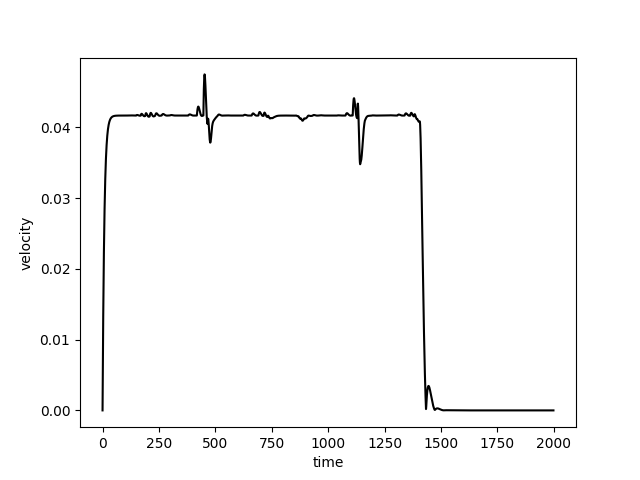
\includegraphics[width=1\linewidth]{master-trajectory-0-velocity}
		\caption{Скорость движения мастера}
		\label{fig:sub2}
	\end{subfigure}
	\caption{Движение мастера по заданной траектории с заданной скоростью $\upsilon_{desired} = 20 \frac{\text{м}}{\text{с}}$. Расстояния на рисунках задаются в метрах, время в секундах, скорость в $\frac{\text{м}}{\text{с}}$}.
	\label{fig:test}
\end{figure}
\subsubsection{Оценка движения мастера по траектории}
Агент преодолел заданную траекторию за $t = 331 \text{с}$. \\
Проеденное расстояние:
$$ S = \int_{0}^{5000} \sqrt{x'^2(s) + y'^2(s)} \ ds \approx 6051 \text{м} $$ \\
Средняя скорость $\upsilon_{av} = 18.3  \frac{\text{м}}{\text{с}}$. \\
Стационарным режимом движения можно назвать режим, при котором скорость агента колеблется в пределах между $18.8\frac{\text{м}}{\text{с}}$ и $21.5\frac{\text{м}}{\text{с}}$. Более подробно скорость мастера в стационарном режиме можно увидеть на рис. \ref{fig:errors-master}a \\

\begin{figure}[!htbp]
	\centering
	\begin{subfigure}{.5\textwidth}
		\centering
		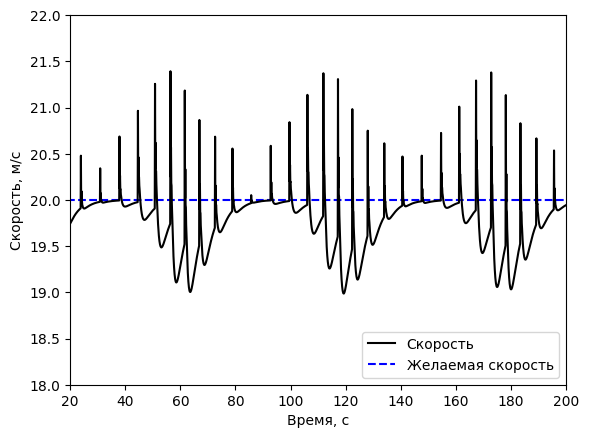
\includegraphics[width=1\linewidth]{master-trajectory-1-velocity.png}
		\caption{Скорость мастера в стационарном режиме}
		\label{fig:error-master-1}
	\end{subfigure}%
	\begin{subfigure}{.5\textwidth}
		\centering
		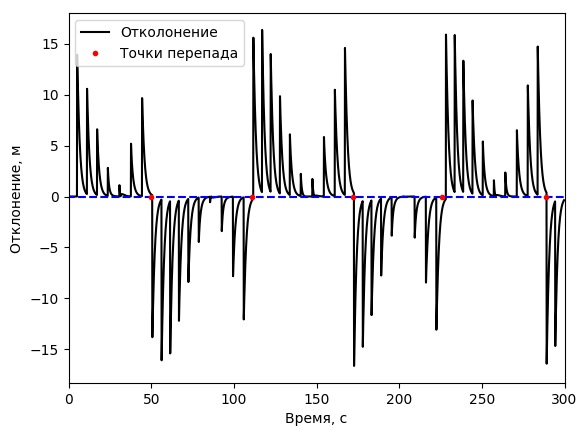
\includegraphics[width=1\linewidth]{master-trajectory-error.png}
		\caption{Отклонения мастера от траектории}
		\label{fig:error-master-2}
	\end{subfigure}
	\caption{Иллюстрация отклонений от желаемого закона движения}.
	\label{fig:errors-master}
\end{figure}
Отклонения агента от заданной траектории представлены на рис. \ref{fig:errors-master}b. Выше нуля — отклонения от траектории вправо, ниже нуля — влево. Максимальное отклонение составляет примерно 15 м. \par
Резкие перепады на графике, обозначенные как точки перепада объясняются тем, что в этих точках у траектории изменяется знак первой производной, а агент, всегда остающийся на внутренней части траектории резко оказывается на внешней. Проверим это утверждение. Заданное выше параметрическое уравнение фактически является уравнением $$x = 300 \cdot \cos(\frac{y}{300})$$
Равенство нулю первой производной:
$$\sin(\frac{y}{300}) = 0 \Rightarrow y = 300 \pi n$$
Найдём первые 5 точек траектории, в которой происходит смена знака второй производной: $$M = \Big\{(-300; \ 942), \ (300; \ 1885), \ (-300; \ 2827), \ (300; \ 3770), \ (-300; \ 4712)\Big\}$$
Найдём моменты времени, в которые эти точки будут достигнуты агентом:
$$\hat{L_t} = \Big\{ 61c, \ 118c, \ 177c, \ 234c, \ 292c \Big\}$$
Реальные же моменты времени, в которые просходит резкое изменение величины отклонения от траектории:
$${L_t} = \Big\{ 50c, \ 110c, \ 172c, \ 226c, \ 289c \Big\}$$
То есть, изменение стороны относительно линии траектории по которой движется агент изменяется незадолго до того, как будет изменён знак первой производной траектории. Эта закономерность так же наблюдается на рис. \ref{fig:master-trajectory-changes-2}. \par
\begin{figure}[!htbp]
	\centering
	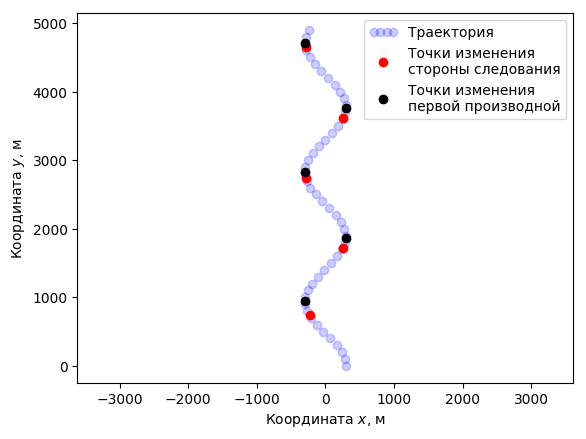
\includegraphics[width=0.5\linewidth]{master-trajectory-changes-2}
	\caption{Траектория с наложенными на неё точками изменения стороны следования и точками изменения знака первой производной.}
	\label{fig:master-trajectory-changes-2}
\end{figure}

\begin{center}{\textit{ (Тут будет исседование устойчивости алгоритма к случайным возмущениям)}}
\end{center}

\subsubsection{Выводы}
Движение мастера по траектории является точным и предсказуемым. Данный алгоритм управления по траектории с задаваемой скоростью является пригодным для применения.

\pagebreak


\subsection{Миньон} \label{minion-section}
Миньон является ведомым агентом, во время движения он никак не использует информацию о траектории движения. Всё, что знает миньон $i$ — это положение своего агента-лидера $L$. Относительно агента-лидера миньон выстраивает свой закон управления $\vec{u_{m}}$: 
$$\vec{u_{m}} = \vec{u_{m}}(L)$$
\par
Более подробно об агентах-лидерах будет сказано в гл. \ref{platoon-section}, а пока о них можно думать просто как о постоянно обновляемой точке, относительно которой агент строит некую другую точку, в которую стремится попасть. Эта точка будет называться виртуальным лидером $L^v$. Точка виртуального лидера своя у каждого миньона и зависит только от реального положения агента-лидера $L$.\par
Пусть, есть миньон с координатами $\vec{A_1}$ и виртуальным лидером в точке $\vec{L_1^v}$. Первый закон управления, который приходит на ум может выглядеть следующим обаразом:
\begin{equation} \label{eq:wrong-controll-minion}
\vec{u_{m}}(t) = S \cdot P \text{, где } S = \big{(}\vec{L_1^v} - \vec{A_1} \big{)}
\end{equation}
\par
Суть такого закона управления в том, что воздействие осуществляется в направлении виртуального лидера с усилием пропорциональным расстоянию между текущей координатой и координатой виртуального лидера. Коэффициент $P$ — пропорциональная составляющая PID регулятора. \par
Однако, такой закон управления не выдерживает некоторых испытаний.
\subsubsection{Воздействие на агента-лидера функцией Хевисайда}
Этот численный эксперимент заключается в следующем: есть пара агентов — миньон и его агент-лидер. На агента-лидера воздействует сила по закону Хевисайда, то есть, фактически, после некоторого момента времени $\hat{t}$ появляется постоянное воздействие на агента-лидера. \par
Для облегчения понимания ситуации рассмотрим воздействие на примере.\par
\begin{figure}[h]
	\centering
	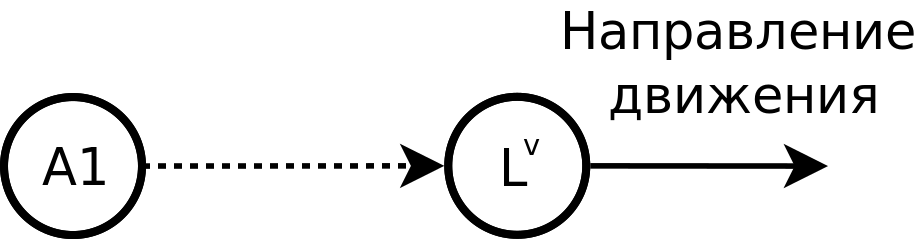
\includegraphics[width=0.4\linewidth]{minion/heviside_struct}
	\caption{}
	\label{fig:hevisidestruct}
\end{figure}
На рис. 4 изображён миньон $A_1$ и его виртуальный лидер $L^v$. На $L^v$ действует сила (распределённая как функция Хевисайда):
$$
F(t) = \begin{cases} 
1 \text{, если $t \geq 5$c} \\
0 \text{, в остальных случаях} \end{cases}
$$

Если использовать закон управления, записанный уравнением (\ref{eq:wrong-controll-minion}), то возникнет ситуация, при которой расстояние между миньоном и его виртуальным агентом будет постоянно расти. Ускорение лидера будет расти быстрее, чем ускорение миньона из-за того, что агент строит свой закон управления только на основании положения лидера, ничего не зная о его ускорении и скорости. Однако передавать эти данные от лидера к миньону может оказаться слишком накладно, т.к. придётся поддерживать более широкий канал связи.
\par
В качестве альтернативы миньон может использовать уже имеющиеся данные о положениях виртуального лидера и увеличивать управляющее воздействие, если расстояние между ним и лидером растёт $\dot{S}$. Так же для устранения статических ошибок добавляется $I$ составляющая PID регулятора.
\begin{equation} \label{eq:right-controll-minion}
\vec{u_{m}}(t) = P \cdot S  + I \cdot \int_0^t{S}dt + D \cdot \dot{S}
\end{equation}
Результаты численного моделирования с данным законом управления:\par
\begin{figure}[!htbp]
	\centering
	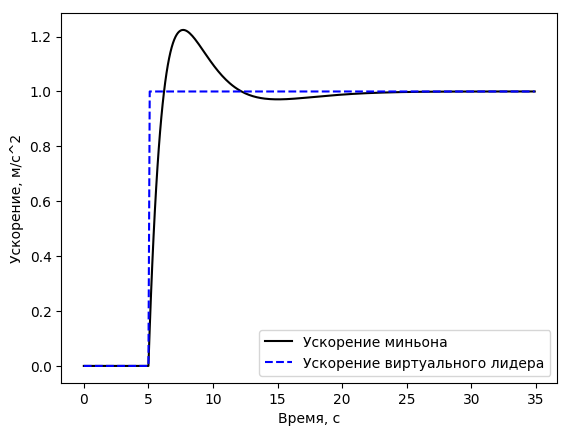
\includegraphics[width=0.6\linewidth]{minion/heviside_accelerations}
	\caption{Ускорение миньона и его виртуального лидера. Вирутальный лидер ускоряется по закону Хевисайда. Ускорение выходит на стационарный режим на 25с: через 20с. после воздействия.}
	\label{fig:hevisideaccelerations}
\end{figure}

\begin{figure}[!htbp]
	\centering
	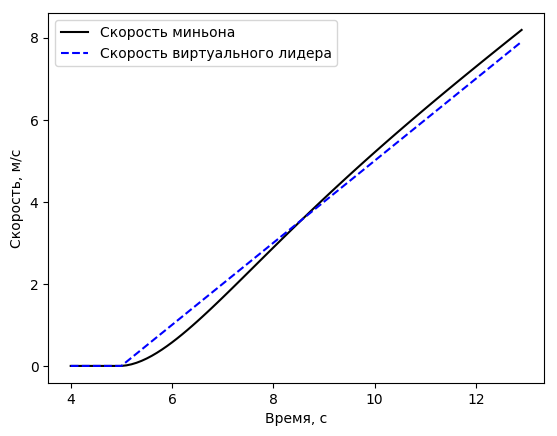
\includegraphics[width=0.6\linewidth]{minion/heviside_velocity}
	\caption{Скорость миньона и виртуального лидера}
	\label{fig:hevisidevelocity}
\end{figure}
\begin{figure}
	\centering
	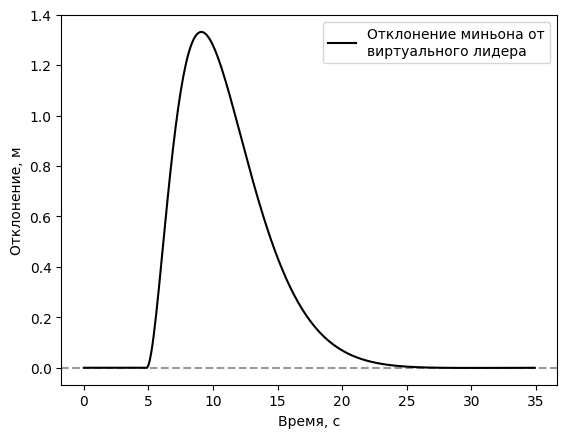
\includegraphics[width=0.6\linewidth]{minion/heviside_targerr}
	\caption{Отклонение положения миньона от его виртуального агента}
	\label{fig:hevisidetargerr}
\end{figure}




\begin{figure}[!htbp]
	\centering
	\begin{subfigure}{.5\textwidth}
	\centering
	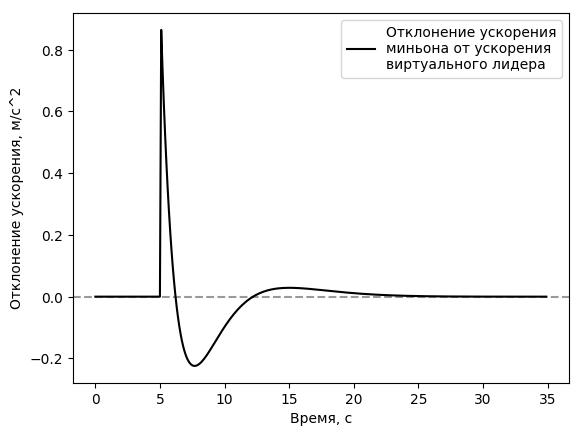
\includegraphics[width=1\linewidth]{minion/heviside_axerr}
	\caption{Отклонение ускорения}
	\label{fig:hevisideaxerr}
	\end{subfigure}%
	\begin{subfigure}{.5\textwidth}
	\centering
	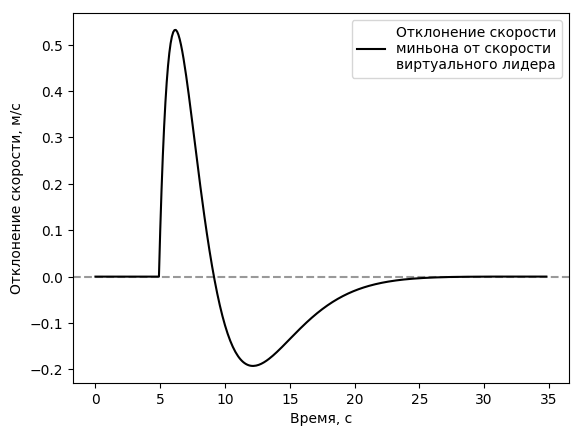
\includegraphics[width=1\linewidth]{minion/heviside_velerr}
	\caption{Отклонение скорости}
	\label{fig:hevisidevelerr}
	\end{subfigure}
	\caption{Иллюстрация отклонений от закона движения виртуального лидера. Выше нуля — значение меньше, чем у лидера, ниже нуля — выше, чем у лидера.}
	\label{fig:errors-minion-heviside}
\end{figure}
\subsubsection{Выводы}
Описанный закон управления справляется с задачей приведения миньона в точку вирутального лидера и будет использован в дальнейшем для управления строем.

\section{Строй} \label{platoon-section}

Строй представляет из себя множество агентов соединённых связями, подобно графу. Для каждого агента, не являющегося мастером должно быть определено не менее одного агента-лидера. Лидером для агента может быть как мастер, так и любой миньон. Каждый агент — вершина графа, каждая связь миньон-лидер — ребро графа. Пример строя из 5-ти агентов изображён на рис.\ref{fig:wedge-platoon}. \par
\begin{figure}[!htbp]
	\centering
	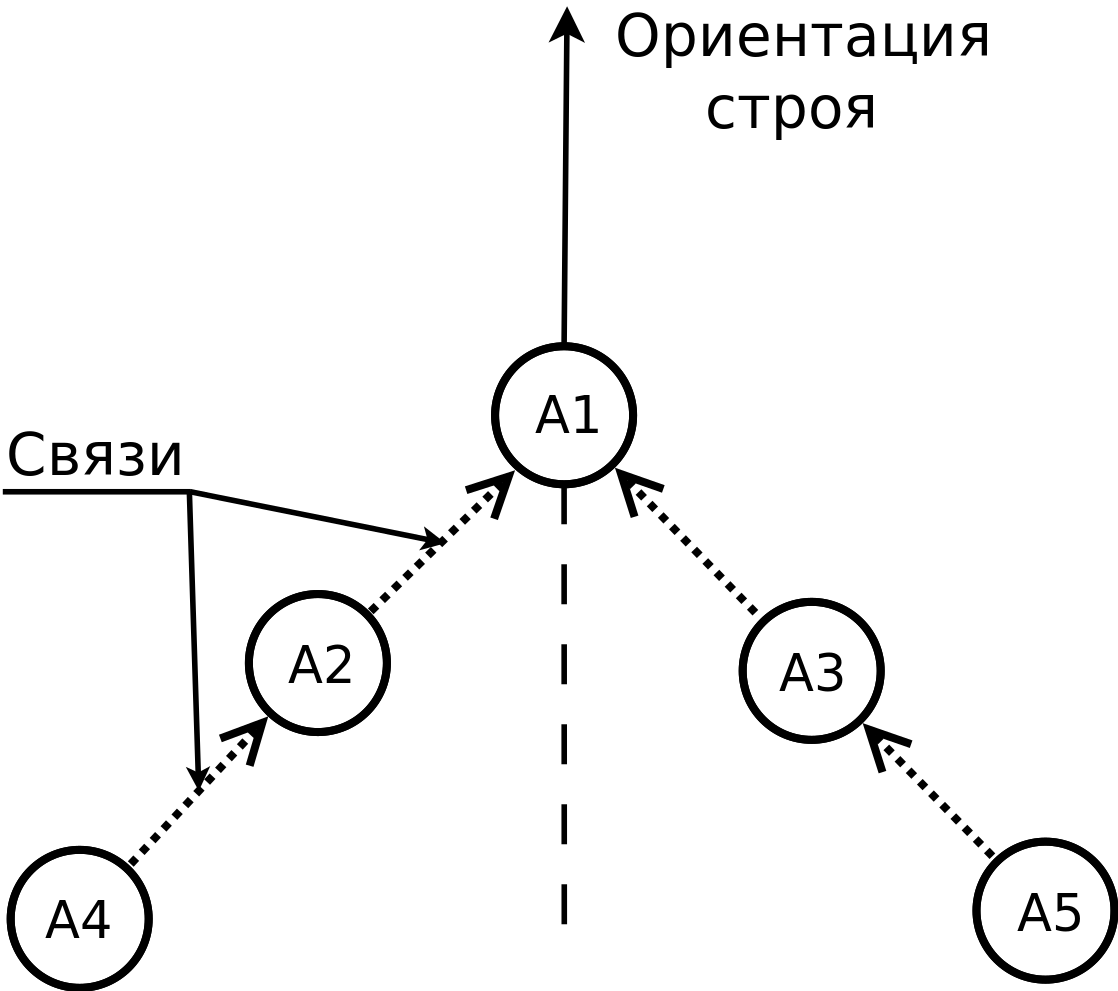
\includegraphics[width=0.5\linewidth]{platoon/wedge-platoon}
	\caption{Пример клиновидного строя из 5-ти агентов}
	\label{fig:wedge-platoon}
\end{figure}
Каждая связь $J_{ij}$ — это вектор в полярных координатах, у которого радиус — это расстояние от миньона $i$ до миньона лидера $j$, а угол — это угол между изначальной ориентацией строя и вектором, соединяющим миньона с его лидером. К примеру, если расстояния между каждой парой агентов равно 1м, то связи:
\begin{itemize}
	\item $J_{1j}$ — не определены ни для каких $j$: $A_1$ является мастером
	\item $J_{21} = (r=1\text{м}; \varphi=225\text{\textdegree{}})$ — для миньона $A_2$ агентом лидером является мастер $A_1$. Агенты находятся на расстоянии 1м, угол между соединяющим их вектором и вектором изначальной ориентации составляет $225 \text{\textdegree}$
	\item $J_{31}, J_{42}, J_{53}$ — определяются аналогично
\end{itemize}
При повороте строя поворачивается и вектор ориентации строя, за счёт чего далее пересчитывается позиция, в которой должен находиться агент после поворота. Эта позиция будет именоваться виртуальным лидером. Виртуальный лидер — точка пространства, в которую стремиться попасть миньон для того, чтобы поддерживать фигуру строя. \par
Например, на рис. \ref{fig:wedge-platoon-rotation} изображён поворот строя на угол $b$. Для того, чтобы пересчитать позицию, в которой должен находиться миньон после поворота (виртуальный лидер) необходимо повернуть вектор изначальной ориентации $O_{0}$ на угол $b + \varphi$, где $\varphi$ — угол из любого вектора связи $J_{ij}$ миньона $i$, далее от положения выбранного миньона-лидера необходимо отложить расстояние равное $r$ из вектора связи в направлении повёрнутого вектора изначальной ориентации $O_0$. 
\par
\begin{figure}[!htbp]
	\centering
	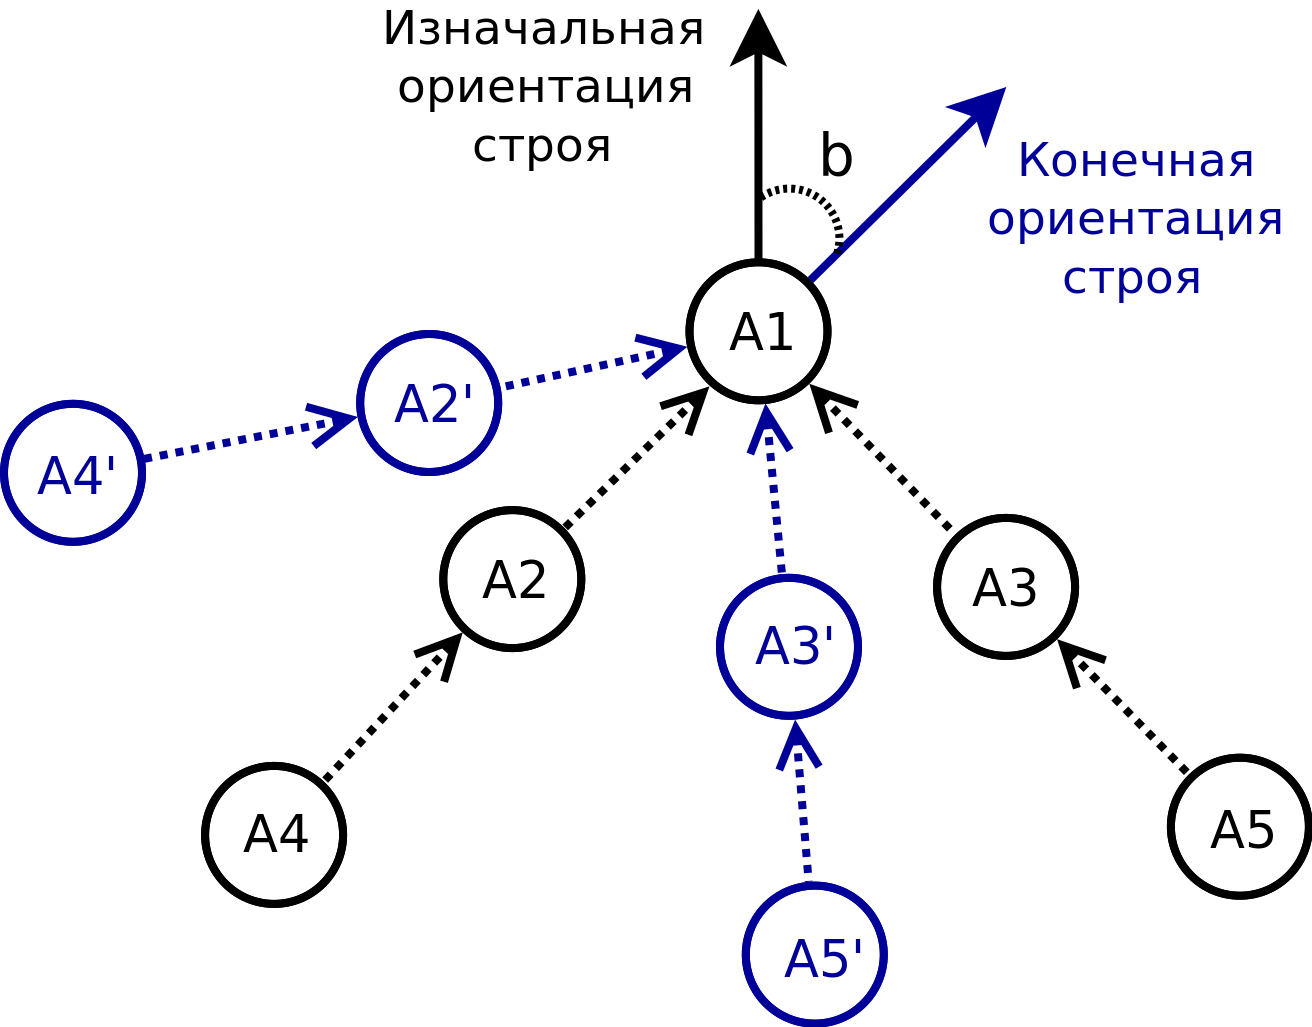
\includegraphics[width=0.5\linewidth]{platoon/wedge-platoon-rotation}
	\caption{Поворот строя на угол $b$}
	\label{fig:wedge-platoon-rotation}
\end{figure}
Рассмотрим пример того, как будет расчитан виртуальный лидер $A_5'$ для агента $A_5$ (см. рис. \ref{fig:wedge-platoon-rotation}), для которого определён вектор связи $J_{53} = (r_{53}; \ \varphi_{53})$ (вектор связи с $A_3$). Для начала повернём вектор изначальной ориентации $O_{0}$:
$$\vec{O_{1}} =  \left(\begin{array}{cc} \cos{(b + \varphi_{53})} & \sin{(b + \varphi_{53})}\\ \sin{(b + \varphi_{53})} & \cos{(b + \varphi_{53})} \end{array}\right) \vec{O_{0}} $$
Теперь вдоль полученного вектора $\vec{O_1}$ необходимо отложить от позиции агента $A_3$ расстояние равное $r_{53}$:
$$ \vec{A'_{5}} = \vec{A_3} + \frac{\vec{O_1}}{|\vec{O_1}|} r_{53}$$
\par
В приведённых выше расчётах неявно предполагалось, что агент $A_3$ на момент пересчёта виртуального лидера для $A_5$ уже находится в точке $A'_3$. До тех пор, пока не будет выполнено это условие получаемое $A'_5$ не будет совпадать с тем, что приведено на рисунке. Однако, это ожидаемая ситуация, т.к. $A_5$ не знает ни о каких агентах кроме $A_3$, то он и полагается только на данные, получаемые от $A_3$, а если $A_3$ ещё не достиг точки виртуального лидера, то и в координтах виртуального лидера $A'_5$ будут содержаться ошибки. \par
Описанную выше проблему несложно решить, если строить виртуальных лидеров на основе позиции не агента-лидера, а на основе точки виртуального лидера агента-лидера. Однако, после поворота у миньонов находящихся дальше от центра поворота (центр поворота — мастер) расстояние до их виртуальных лидеров окажется больше, чем у миньонов ближе к центру поворота (см. $A_3$ — $A'_3$ в сравнении с $A_5$ — $A'_5$ на рис. \ref{fig:wedge-platoon-rotation}), что приведёт к тому, что пропорциональная составляющая $PID$ регулятора вырабатывающего управление для следования миньонов в точку виртуального лидера выдаст команду создать большее управляющее воздействие, следовательно АКБ агентов будут разряжаться более неравномерно, чем при более инертном рассчёте виртуальных лидеров от позциии агентов-лидеров.
\subsection{Моделирование движения строя}


\begin{figure}[!htbp]
	\centering
	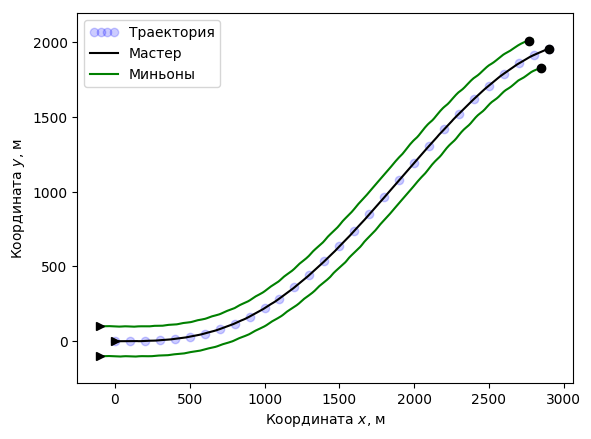
\includegraphics[width=0.7\linewidth]{platoon-trajectory-0}
	\caption{Движение строем мастера и двух миньонов}
	\label{fig:platoon-trajectory-0}
\end{figure}


\end{document}